\section{Construction}\label{sec:construction}

Before diving into the details of the pseudocode, we give an intuitive overview
of the \rollerblade construction.

% TODO: Consider whether there is duplication with the introduction here

There are $m$ \rollerblade clients numbered $1, 2, \ldots, j, \ldots, m$
and $n$ underlying protocols $\Y[][1], \Y[][2], \ldots, \Y[][i], \ldots, \Y[][n]$.
Each $\RB[j]$ of the clients runs a full node for each of the $n$ underlying
ledger protocols,
$\Y[j][1], \Y[j][2], \ldots, \Y[j][i], \ldots, \Y[j][n]$.
Each $\RB[j]$ \emph{simulates} within its implementation $n$ different instances
of the overlay protocol $\Pi$,
$\Z[j][1], \Z[j][2], \ldots, \Z[j][i], \ldots, \Z[j][n]$,
one for every underlying ledger protocol,
$\Y[j][1], \Y[j][2], \ldots, \Y[j][i], \ldots, \Y[j][n]$.
% TODO: figure

The \rollerblade client $\RB[j]$ allows the external user to issue a \emph{write} instruction
to any $i^\text{th}$ simulated machine $\Z[j][i]$. This is done as follows. When the user
of $\RB[j]$ issues a \emph{write} instruction to $\Z[j][i]$, this instruction is not given to
$\Z[j][i]$ directly. Instead, it is \emph{encoded} into a transaction and recorded on the
respective underlying ledger $\Y[j][i]$.
The encoding functionality is made available because
the underlying ledgers are assumed to be bulletin boards.
When the `write' instruction becomes recorded in the ledger $\Ledger[j][i]$ reported
by $\Y[j][i]$, then it will be passed to the simulated
machine $\Z[j][i]$ as soon as the respective round simulation takes place.
Through this recording of machine inputs on-ledger, we intent for other
rollerblade clients $\RB[j']$ to replicate the exact simulation of $\Z[j'][i]$ for that
same $i$ (in the Analysis section, this is made precise in Conjecture~\ref{conj:cross-party}).
Additionally, the external user can, at any time, issue a \emph{read} instruction to
the simulated machine $\Z[j][i]$, without affecting its current state (recall that we
require $\Pi$'s \emph{read} method to not alter the machine's internal state upon completion).

Each of $\Z[j][i]$ is simulated in a per-round basis by having its \emph{execute}
function invoked once per round $r$. When it is simulated, it expects its \emph{write} function to have
been called some ($0$ or more) number of times prior to \emph{execute} being invoked,
indicating user input for round $r$. When \emph{execute} is invoked, it has access to read
and write into the network through the authenticated channels interface $\net$.
When it \emph{reads} from the network, it consumes network messages that other machines
have dispersed into the network during previous rounds (potentially with some delay $\Delta$).

In order to simulate this communication between machines, the system works as follows.
A \emph{relayer} node is tasked with \emph{checkpointing} every ledger to every other ledger
during every round. There is no trust placed upon this relayer, but at least one relayer
is assumed to be honest (a client can run its own relayer if it so wishes, so this does
not introduce any additional trust assumptions). Checkpointing is performed as follows.
The relayer runs a full node in each of the underlying protocols $\Y[][i]$ and
invokes the \emph{transcribe} function $\Y[][i].\transcribe()$ to obtain a transcription
$\tau$; this functionality is made available because underlying ledgers are assumed to be
transcribable. This transcription is then checkpointed into every other ledger protocol
$\Y[][i']$ by \emph{encoding} it into a bulletin transaction $\tx = \Y[][i'].\encode(\tau)$
and \emph{writing} it into $\Y[][i']$. The relayer is illustrated in
Algorithm~\ref{alg.relayer}.

\emph{These ``write'' and ``checkpoint'' instructions are the only thing ever written
to the ledger from the honest rollerblade clients}. In particular, no network outputs
produced by any of the $\Z[j][i]$ are ever written on the ledger. Instead, we observe
that reading the checkpoints is sufficient for each rollerblade client to reproduce
the network outputs of all simulated machines.

Let us now explore, in more detail, how this simulation works.

% \subsection{A Majority Vote}\label{sec:construction-naive}
%
% Composing many underlying ledgers into an overlay ledger is not complicated, but it is complex
% protocol, with many moving parts. As such, we present the design in iterative stages. In the
% first stage, presented in the present section, we provide a design based on an \emph{honest majority}
% approach. This obvious approach introduces the notation and allows us to familiarize the reader
% with the concepts, but is ultimately misguided. However, it is imperative for understanding why
% a straightforward solution is not applicable, and a stepping stone for the next development in
% the protocol. In the section that follows, we introduce a BFT layer running on top of our
% underlying ledgers. This is our final construction, but we describe it intuitively first before
% we delve into the technical details of a precisely defined construction in the next section.
% We leave the formal analysis and proofs of security for the end.
%
% The first and obvious approach to compose ledgers starts by the assumption that the
% underlying majority is secure. The core idea is to produce the overlay ledger by taking
% a majority vote on the reported underlying ledgers. The construction is illustrated in
% Figure~\ref{fig.naive}, where
% $m$ parties $\RB[1], \ldots, \RB[m]$ run the overlay protocol.
% Each of the $\RB$ nodes runs
% a full node to each of the $n$ underlying DLPs $\wheel[1], \ldots, \wheel[n]$, pictured as squares
% of varying shades of yellow. The full nodes communicate with one another using their
% respective DLP technology, which we treat as a black box here, depicted as elongated
% rectangles in varying shades of red towards the bottom of the figure.
% The $\RB$ nodes
% make their own overlay DLP, offering \emph{read} and \emph{write} functionalities.
%
% \begin{figure*}
%     \centering
%     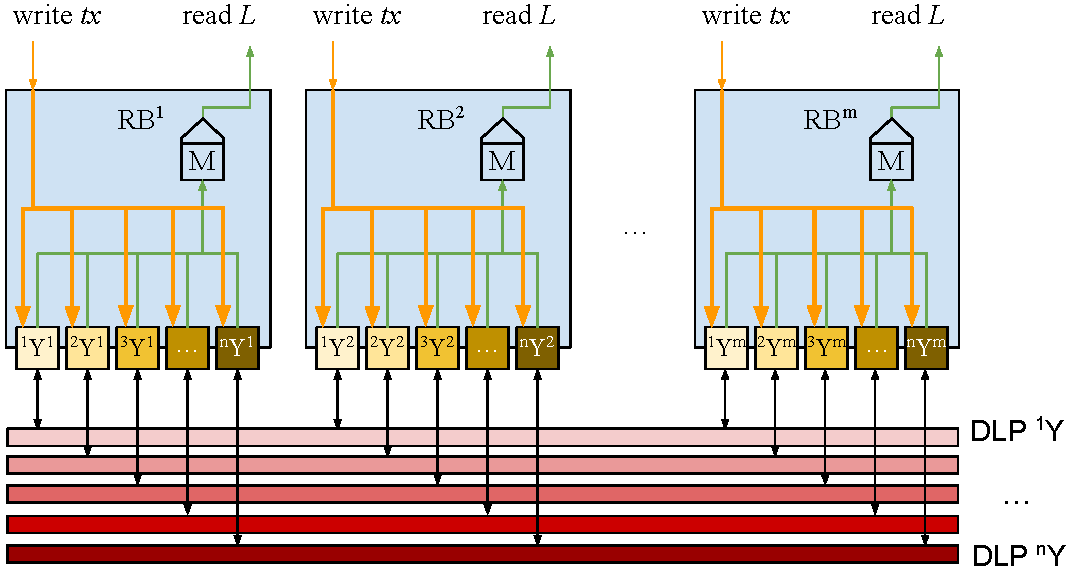
\includegraphics[width=\textwidth,keepaspectratio]{figures/rollerblade-naive-construction.pdf}
%     \caption{The first attempt at the composed construction. Here,
%              $m$ different parties $\RB_1, \ldots, \RB_m$ operate Rollerblade
%              nodes, each of which runs a client on $n$ different underlying
%              DLPs $Y_1, \ldots, Y_n$.}
%     \label{fig.naive}
% \end{figure*}
%
% When an $\RB$ transaction $\tx$ is \emph{written} into one of the $\RB$ nodes by the user,
% the $\RB$ serializes this transaction for each of the underlying DLPs (using the
% serialization mechanism particular to each individual DLP) and posts it
% as a transaction there, depicted as orange wires running downwards in the figure.
% Let us walk through
% this process precisely.
% The $\RB$ party takes $\tx$ and wraps it in a \emph{message}
% which is the pair $m = (`\text{write}', \tx)$.
% This captures the user intent to \emph{write} this overlay transaction to the underlying ledgers.
% The first element of the pair (\emph{`write'}) indicates the \emph{type} of message.
% As we evolve our protocol, we will introduce other control message types later, but,
% for now, this is our only message type. Once the message is created, we pass it to
% \textsf{encodeRollerbladeTx}, listed in Algorithm~\ref{alg.encode}.
% This function first serializes $m$
% into a string $s = \textsf{serialize}(m)$. This string is then encoded for each particular
% underlying DLP $\wheel[i]$ by invoking the bulletin functionality $\wheel[i]\text{.encode}$.
% This returns a transaction $\tx'_j$, which is appropriate for being written to $\wheel[i]$.
% Note that $\tx$ is a transaction of the overlay ledger, whereas each of $\tx'_i$ is a
% transaction of the underlying ledger $\wheel[i]$. Each resulting underlying transaction $\tx'_i$
% is then broadcast into $\wheel[i][j]$ by having $\RB[j]$ invoke the \emph{write}
% functionality of $\wheel[i][j]$.
%
% \import{./}{algorithms/alg-encode}
%
% Each transaction $\tx'_i$ is written to the respective underlying DLP $\wheel[i][j]$ during
% the same round $r$. If $i$ happens to be live, the respective \emph{read} call of all
% other $j'$ DLPs on $\wheel[i][j']$ at round $r' \geq r + u$ will result in a ledger
% $\wheel[i][j'][r']$ containing $\tx'_i$.
%
% In order to answer a particular overlay \emph{read} call, the overlay party $\RB[j']$ must
% issue a \emph{read} to all of its underlying DLPs $\wheel[1][j'], \ldots, \wheel[n][j']$,
% depicted as green wires running upwards in the figure.
% The transactions in $\wheel[i][j'][r']$ are of $\wheel[i]$ format,
% and therefore must be decoded using the bulletin decoding functionality
% appropriate to each underlying DLP $\wheel[i]$.
% Those that decode successfully result in a string $s$ which can, in turn,
% be deserialized into a message $m = (`write', \tx)$ containing the type \emph{`write'}
% and the overlay transaction $\tx$. The process of decoding and deserializing a transaction
% is done through the \textsf{decodeRollerbladeTx} algorithm, listed in Algorithm~\ref{alg.encode}.
% It invokes \textsf{decodeRollerbladeTx} in each of the returned ledgers, resulting
% in a sequence of $n$ ledgers $\overline{L}$, each a sequence of overlay transactions.
% We call this process \emph{sanitization} and list it in Algorithm~\ref{alg.sanitize}.
%%
% Next, the overlay party $\RB[j']$ will need a mechanism to combine these sanitized ledgers
% into \emph{one} ledger in order to answer the \emph{read} call from the user.
% The sanitized ledgers are fed into a \emph{majority voting} contraption, denoted with
% the letter M and the \emph{house} symbol in the figure, which then outputs the desired
% ledger $L$ of $\RB$ transactions (top).
% The idea is that, if the majority of underlying ledgers is secure, the transaction $\tx$
% in question will eventually appear (liveness) and stabilize (safety) in a majority of them.
% The party $\RB[j']$ can therefore take a majority vote among the underlying ledgers
% to extract an overlay ledger aspiring to be safe and live.
% The algorithm listed in Algorithm~\ref{alg.majorityvote} performs the majority voting
% process. It is invoked when the user of $\RB[j]$ invokes \emph{read} at a certain
% round $r$. The process accepts a list of ledgers $\overline{L}$ each $\prescript{i}{}{\overline{L}}$
% of which contains the sanitization of the underlying ledger $\wheel[i][j][r]$.
% The majority of $\overline{L}$ will contain all the honest
% transactions issued at least $u$ rounds ago. It goes through each
% position in the sanitized ledgers. For each position $k \in \mathbb{N}$,
% it observes what each of the $n$ ledgers report in the $k^\text{th}$ position.
% The reported transactions in the $k^\text{th}$ position are
% $\wheel[1][j][r][k], \wheel[2][j][r][k], \ldots, \wheel[n][j][r][k]$.
% The algorithm counts the frequency of appearance of each transaction at
% the position $k$. If a transaction
% appears more than $\frac{n}{2}$ times in this position, it is included in the sanitized ledger
% (since we have $n$ underlying ledgers, only one transaction can do so).
% Otherwise, if no transaction appears more than $\frac{n}{2}$, the sanitized ledger
% is cut short and returned.
%
% \import{./}{algorithms/alg-majorityvote}
%
% The intuition why this majority voting \emph{should work} is this: An honest
% transaction will eventually be included in all of the underlying ledgers that
% are live, and hence will appear in more than $\frac{n}{2}$ underlying ledgers
% and will make it to the output of \textsf{MajorityVote}. Since the majority
% of underlying ledgers is secure, they will maintain the transaction order,
% and so will the output of \textsf{MajorityVote}. In order for the adversary
% to censor a transaction from the final ledger, the adversary will need to
% break the security of more than $\frac{n}{2}$ underlying ledgers.
%
% Unfortunately, this argument does not hold water. The reason is that, due to
% delays, two transactions $\tx_1$ and $\tx_2$ may appear in a different order
% in different underlying ledgers, even if all of them are secure. It is possible
% that $\tx_1$ appears before $\tx_2$ in $\lfloor \frac{n}{2} \rfloor$ of the
% underlying ledgers, whereas it appears after $\tx_2$ in the $\lceil \frac{n}{2} \rceil$
% of the rest\footnote{In fact, it is possible, even with every underlying ledger being
% secure, that each ledger reports a particular order of transactions, but the majority voting
% cannot not result in an order at all. This is known as a Condorcet cycle~\cite{condorcet}.}.
% The adversary can then easily swap the transaction order by
% breaking the security of only one chain. Therefore, this initial design
% is not secure. We are now ready to rectify this issue by introducing a more
% nuanced mechanism in place of majority voting.
%
% \subsection{A BFT to Rule Them All}\label{sec:construction-bft}
%
% \begin{itemize}
%   \item Simple majority voting construction with no BFT protocol on top. Serialization and deserialization requirements and algorithms. Majority voting on ``ledger extensions'' algorithm. Fragile results in which different blockchains can disagree on the order and one blockchain can ``flip over'' the result. l. Condorcet cycles.
%   \item The necessity of running a BFT protocol on top, but without talking about the oracle abstraction of signatures, broadcasting, verification, and receiving. Light clients from one blockchain to another using smart contracts. Using the blockchains as ports of communication.
%   \item Oraclizing sign/broadcast and receive/verify.
%   \item Remove the smart contract assumption using dirty ledgers.
%   \item The full construction.
% \end{itemize}
%
% \subsection{Compatibility}\label{sec:compatibility}
%

\import{./}{algorithms/alg-relay}
\import{./}{algorithms/alg-decode-underlying}
\import{./}{algorithms/alg-outboxes-to-inbox}
\import{./}{algorithms/alg-prepare-simulation-inputs}
\import{./}{algorithms/alg-simulate}
\import{./}{algorithms/alg-read-write}

%
% \section{New material 2023-04-19}
%
% Known origin oracle.
%
% \import{./}{algorithms/alg-known-origin}
% \import{./}{algorithms/alg-transferable-origin}
%
% \dionyziz{TODO: recursive transferable origin oracle; gossip oracle}
%
% A distributed protocol amendable to the \rollerblade transform must be given as
% an oraclized \emph{deterministic} Turing Machine designed to work with the
% $\fko$ or $\fto$ functionalities as an oracle.
%
% \begin{enumerate}
%   \item Table of analogies: $u$-liveness = $\Delta$-delay; GST = eventual liveness; safety failure = RR failure; party = ledger...
%   \item Rollerblade ledger: A construction of a ledger protocol on top of rollerblade.
% \end{enumerate}
%
% % TODO: Remark: Dolev--Strong can be ran on top of \rollerblade. This is useful when combined with interoperability.
%
